\begin{figure}
  \setlength{\unitlength}{\textwidth}
\fbox{
        \begin{picture}(1,0.5)(0,0.255)

      % % % Parkinson Data 
      \put(0.025,0.5){\includegraphics[width=0.5\unitlength]{../FnP/gnuplot/fqss_fsi_displace.eps}}
      \put(0.5,0.5){\includegraphics[width=0.5\unitlength]{../FnP/gnuplot/qss_fsi_velocity.eps}}
      \put(0.3,0.25){\includegraphics[width=0.5\unitlength]{../FnP/gnuplot/qss_fsi_power.eps}}
      
      



      
      \put(0.45,0.7){\small(a)}
      \put(0.926,0.7){\small(b)}
      \put(0.726,0.45){\small(c)}
  

      
    \end{picture}
}
  \caption{Comparison of data generated using the quasi-static theory and full DNS simulations . (a) Displacement amplitude, (b) velocity amplitude and (c) mean power as functions of \massdamp. Data were
  obtained at Re = 200 and \hilight{pi2 values} }
    \label{fig:qss_fsi}
\end{figure}

 %vspace{10cm}
